\textcolor{red}{写的很难受, 该不该写Data Analysis? 总觉得不对劲}

\section{Data Analysis}
Data analysis is a critical step in understanding the underlying quality, patterns, and characteristics of the dataset.

\subsection{Data Quality Check}
Ensuring high data quality is a critical first step before any analysis. In this stage, the following checks are performed:
\begin{itemize}
    \item \textbf{Missing Values:} Confirm that there are no missing entries, or if there are, decide on an appropriate imputation method.
    \item \textbf{Outliers:} Identify any extreme values using statistical methods (this project used IQR), or if there are any, determine if they need to be removed or capped.
    \item \textbf{Duplicates:} Check for duplicate records to prevent bias in analysis.
    \item \textbf{Consistency and Integrity:} Ensure data types, ranges, and formats are consistent across the dataset.
\end{itemize}

\textbf{Results:} All datasets collected via yfinance contain no missing values or duplicates, and no outliers were detected using the Interquartile Range (IQR) method. Data types are consistent, with the `Date` as an object and `Close` as float64.

\subsection{Exploratory Data Analysis}
Exploratory Data Analysis (EDA) involves summarizing the main characteristics of the dataset using visual and quantitative methods. This project includes the following EDA techniques:
\begin{itemize}
    \item \textbf{Summary Statistics:} Compute mean, median, variance, and other descriptive measures to understand data distribution.
    \item \textbf{Line Chart for Long-Term Trends:} Plot the USDEUR exchange rate over time to reveal long-term trends and identify potential anomalies. (See Figure~\ref{fig:line_chart}.)
    \item \textbf{Rolling Statistics for Volatility Analysis:} Compute the rolling mean and standard deviation of the USDEUR exchange rate using a 30-day window to assess volatility changes over time. (See Figure~\ref{fig:rolling_statistics}.)
\end{itemize}

\begin{figure}[H]
\centering
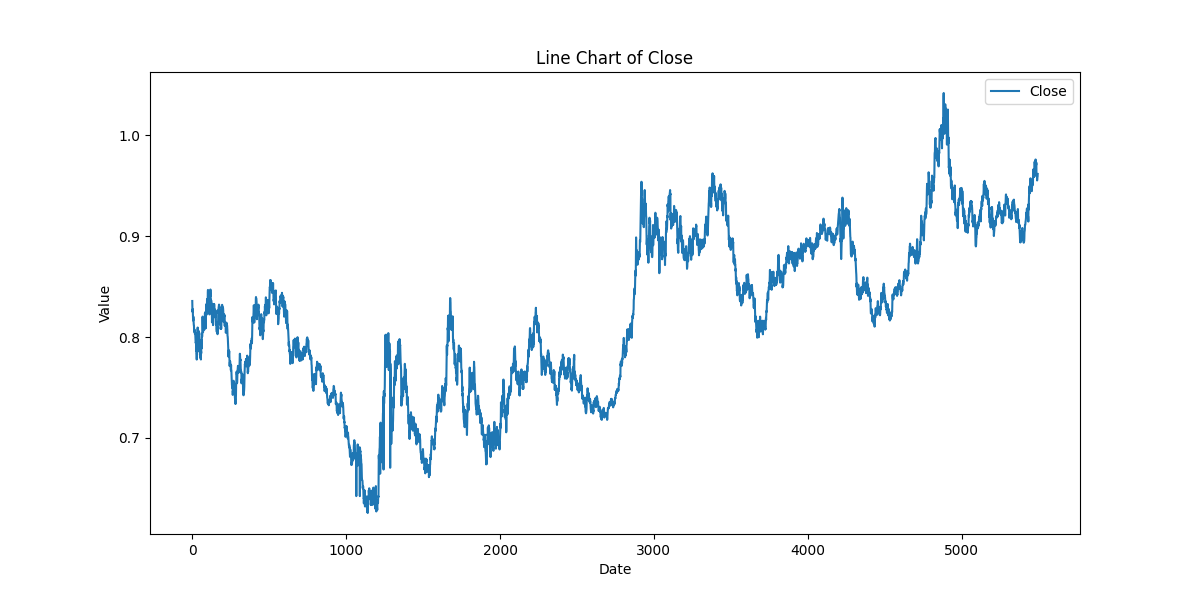
\includegraphics[width=\textwidth]{figures/line_chart}
\caption{Line Chart of the USDEUR Exchange Rate (The Primary Dataset)}
\label{fig:line_chart}
\end{figure}

\begin{figure}[H]
\centering
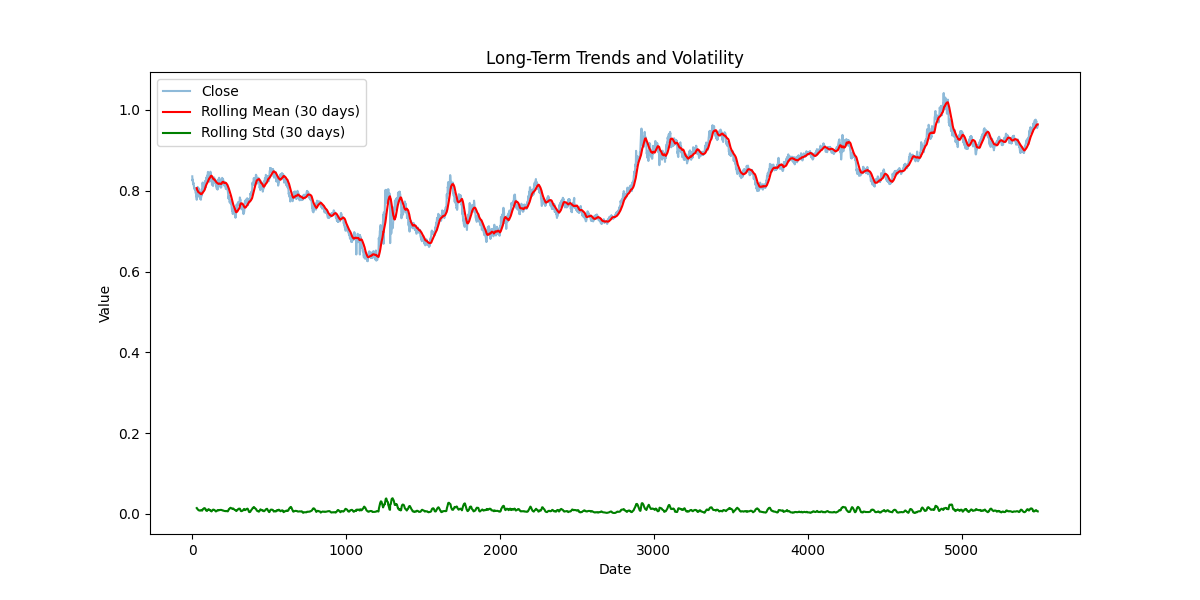
\includegraphics[width=\textwidth]{figures/rolling_statistics}
\caption{Rolling Mean and Standard Deviation of the USDEUR Exchange Rate (The Primary Dataset))}
\label{fig:rolling_statistics}
\end{figure}

For the primary dataset, its summary statistics indicate that the mean exchange rate is approximately 0.823 with a standard deviation of 0.084, which reflects moderate variability. The line charts visually confirms this stability, which highlights long-term fluctuations without evident anomalies.

\subsection{Stationarity Testing}
Stationarity testing is an important process in time series analysis. A stationary time series has statistical properties that do not change over time.

\subsubsection{Augmented Dickey-Fuller Test}
The Augmented Dickey-Fuller (ADF) test operates under the following principles:
\begin{itemize}
    \item \textbf{Null Hypothesis (H\(_0\)):} The time series has a unit root (non-stationary).
    \item \textbf{Alternative Hypothesis (H\(_1\)):} The time series is stationary.
\end{itemize}


\subsubsection{Kwiatkowski-Phillips-Schmidt-Shin Test}
The Kwiatkowski-Phillips-Schmidt-Shin (KPSS) test operates under these principles:
\begin{itemize}
    \item \textbf{Null Hypothesis (H\(_0\)):} The time series is stationary around a deterministic trend (level stationary).
    \item \textbf{Alternative Hypothesis (H\(_1\)):} The time series is non-stationary.
\end{itemize}

\textbf{Results:} The ADF test failed to reject the null hypothesis of a unit root at the 1\% significance level, while the KPSS test rejected the null hypothesis of stationarity at the 1\% level. Together, these results provide strong evidence that the dataset is non-stationary, which suggests that further differencing is required to achieve stationarity.

\textcolor{red}{QUESTION: multivariate的feature selection部分不放在这里有影响吗?}
